% !TeX root = ../tjuthesis-example.tex

\section{排版示例}

这一章中我们给出一些排版示例, 以便一些对\LaTeX 不熟悉的同学来学习参考.
% TODO: 列举 换页

\clearpage
\subsection{插图}

我们先来整理一下手册对插图的要求. 手册中第十九页及第二十页中提到:
\begin{quote}
  毕业设计 (论文) 的插图 (此处插图系指正文中的插图) 必须精心制作, 线条粗细要合适, 图面要整洁美观. 每幅插图应有图序和图题, 图序和图题应放在图位下方居中处. 图序, 图题采用宋体小5号. 图应在描图纸或在白纸上用墨线绘成, 也可以用计算机绘图. 插图上下均应空一行.
\end{quote}
手册中第五十二页的参考例文中提到:
\begin{quote}
  图居中, 上下与正文之间各空一行.
  图中文字: 小五, 宋体 (英文 Times New Roman), 行距1倍, 段前0行, 段后0行.
  插图应有图序和图题, 全文插图以章分组编序号, 图序必须连续, 不得重复或跳缺. 如图4.1表示第四章的第一幅图.
  图题: 小五, 宋体 (英文 Times New Roman), 居中置于图下方, 行距18磅, 段前0行, 段后0行.
\end{quote}

现在我们应该来说一下应该如何插图. 我们在文档类中已经引用了\pckg{graphicx}包. 我们拿手册中的插图作为示例.

\begin{figure}[htb]
  \centering
  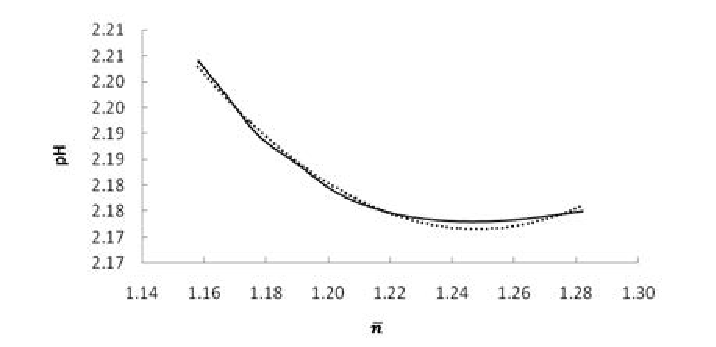
\includegraphics{figures/oxalic-acid-n-geq-1.15.pdf}
  \caption{乙二酸$\overline{n}\geq 1.15$数据段曲线及其拟合曲线 (实线--实际曲线, 虚线--拟合曲线) 乙二酸$\overline{n}\geq 1.15$数据段曲线及其拟合曲线 (实线--实际曲线, 虚线--拟合曲线) 乙二酸$\overline{n}\geq 1.15$数据段曲线及其拟合曲线 (实线--实际曲线, 虚线--拟合曲线)}
\end{figure}

\zhlipsum[1]
